\documentclass[tikz, border=10pt]{standalone}
\usepackage{tikz}
\usetikzlibrary{calc}

\begin{document}
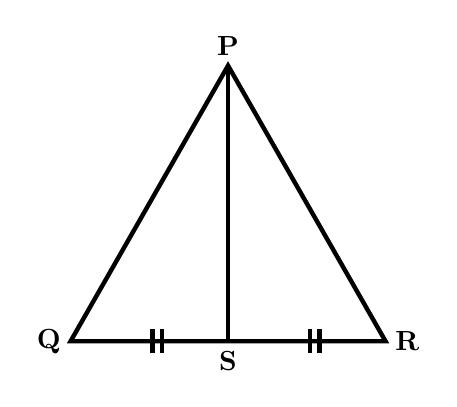
\begin{tikzpicture}

% Define vertices of the triangle
\coordinate (P) at (2, 3.5);
\coordinate (Q) at (0, 0);
\coordinate (R) at (4, 0);

% S is the midpoint of QR
\coordinate (S) at ($(Q)!0.5!(R)$);

% Draw the triangle PQR
\draw[ultra thick] (P) -- (Q) -- (R) -- cycle;

% Draw the line PS (median)
\draw[ultra thick] (P) -- (S);

% Tick mark on QS (midpoint of QS)
\coordinate (M1) at ($(Q)!0.47!(S)$);
\draw[ultra thick] ($(M1)+(0.1, 0.15)$) -- ($(M1)+(0.1, -0.15)$);
% Tick mark on QS (midpoint of QS)
\coordinate (M2) at ($(Q)!0.53!(S)$);
\draw[ultra thick] ($(M2)+(0.1, 0.15)$) -- ($(M2)+(0.1, -0.15)$);


% Tick mark on SR (midpoint of SR)
\coordinate (M3) at ($(S)!0.47!(R)$);
\draw[ultra thick] ($(M3)+(0.1, 0.15)$) -- ($(M3)+(0.1, -0.15)$);
\coordinate (M4) at ($(S)!0.53!(R)$);
\draw[ultra thick] ($(M4)+(0.1, 0.15)$) -- ($(M4)+(0.1, -0.15)$);

% Labels
\node[above] at (P) {\textbf{P}};
\node[left] at (Q) {\textbf{Q}};
\node[right] at (R) {\textbf{R}};
\node[below] at (S) {\textbf{S}};

\end{tikzpicture}
\end{document}